\section{Digital Filter Realizations (Chapter 7)}

%%%%%%%%%%%%%%%%%%%%%%%%%%%%%%%%%%%%%%%%%%%%%%%%%%%%%%%%%%%%
\subsection{Equivalent Descriptions of Digital Filters}

Ein diskretes LTI-System kann äquivalent beschrieben werden durch:

\begin{itemize}
\item Impulsantwort $h(n)$
\item Faltung: $y(n)=h(n)*x(n)$
\item Transferfunktion $H(z)$
\item Frequenzgang $H(e^{j\omega})$
\item I/O-Differenzgleichung
\item Blockdiagramm (Realisierungsform)
\end{itemize}

Zusammenhang:

\[
H(z)=\sum_{n=-\infty}^{\infty} h(n)z^{-n}
\]

\[
H(e^{j\omega}) = H(z)\big|_{z=e^{j\omega}}
\]

Designablauf:

\begin{enumerate}
\item Spezifikation (Passband, Stopband, Ordnung)
\item Bestimmung von $H(e^{j\omega})$
\item Approximation → rationales $H(z)$
\item Wahl einer Realisierungsstruktur
\end{enumerate}

Wichtig:  
Alle Realisierungsformen besitzen dieselbe Transferfunktion, unterscheiden sich jedoch in:
\begin{itemize}
\item Speicherbedarf
\item Anzahl Operationen
\item Numerischer Robustheit
\end{itemize}

%%%%%%%%%%%%%%%%%%%%%%%%%%%%%%%%%%%%%%%%%%%%%%%%%%%%%%%%%%%%
\subsection{Transfer Function}

Allgemeine rationale Form:

\begin{equation}
H(z)=\frac{Y(z)}{X(z)}=
\frac{b_0+b_1z^{-1}+...+b_Lz^{-L}}
{1+a_1z^{-1}+...+a_Mz^{-M}}
\end{equation}

Ordnung des Systems:
\[
\text{ord}(H)=M
\]

Pole:
\[
D(z)=0
\]

Zeros:
\[
N(z)=0
\]

Stabilitätsbedingung (BIBO):
\[
|p_i|<1
\]

%%%%%%%%%%%%%%%%%%%%%%%%%%%%%%%%%%%%%%%%%%%%%%%%%%%%%%%%%%%%
\subsection{Herleitung der I/O-Differenzgleichung}

Aus

\[
H(z)=\frac{Y(z)}{X(z)}
\]

folgt:

\[
\left(1+\sum_{k=1}^{M} a_k z^{-k}\right)Y(z)
=
\left(\sum_{k=0}^{L} b_k z^{-k}\right)X(z)
\]

Inverse $z$-Transformation:

\[
y(n)+\sum_{k=1}^{M} a_k y(n-k)
=
\sum_{k=0}^{L} b_k x(n-k)
\]

Isolieren von $y(n)$:

\begin{equation}
y(n)
=
-\sum_{k=1}^{M} a_k y(n-k)
+
\sum_{k=0}^{L} b_k x(n-k)
\end{equation}

Interpretation:

\begin{itemize}
\item $b_k$ → Feedforward (Zeros)
\item $a_k$ → Feedback (Poles)
\item Vorzeichenwechsel bei $a_k$
\end{itemize}

%%%%%%%%%%%%%%%%%%%%%%%%%%%%%%%%%%%%%%%%%%%%%%%%%%%%%%%%%%%%
\subsection{Impulsantwort}

Für $x(n)=\delta(n)$:

\[
h(n)=y(n)
\]

Rekursive Berechnung:

\[
h(n)=
-\sum_{k=1}^{M} a_k h(n-k)
+
b_n
\]

mit

\[
b_n=
\begin{cases}
b_n & 0\le n\le L \\
0 & n>L
\end{cases}
\]

Initialbedingungen:

\[
h(n)=0 \quad \text{für } n<0
\]

\subsubsection*{Spezialstruktur $1-z^{-N}$}

\[
H(z)=\frac{B(z)}{1-z^{-N}}
\]

Da

\[
\frac{1}{1-z^{-N}}=\sum_{k=0}^{\infty} z^{-kN}
\]

ergibt sich:

\[
h(n)=h(n-N)+b(n)
\]

$\Rightarrow$ Impulsantwort ist periodisch mit Periode $N$.

%%%%%%%%%%%%%%%%%%%%%%%%%%%%%%%%%%%%%%%%%%%%%%%%%%%%%%%%%%%%
\subsection{Direct Form I}

Direkte Umsetzung der Differenzgleichung.

Struktur:

\begin{itemize}
\item Eine Delay-Kette für $x(n)$
\item Eine Delay-Kette für $y(n)$
\end{itemize}

Speicherbedarf:
\[
L+M
\]

Algorithmus:

\begin{enumerate}
\item Berechne
\[
y(n)= -\sum_{k=1}^{M} a_k y(n-k)
+ \sum_{k=0}^{L} b_k x(n-k)
\]
\item Zustände in umgekehrter Reihenfolge aktualisieren
\end{enumerate}

\begin{center}
    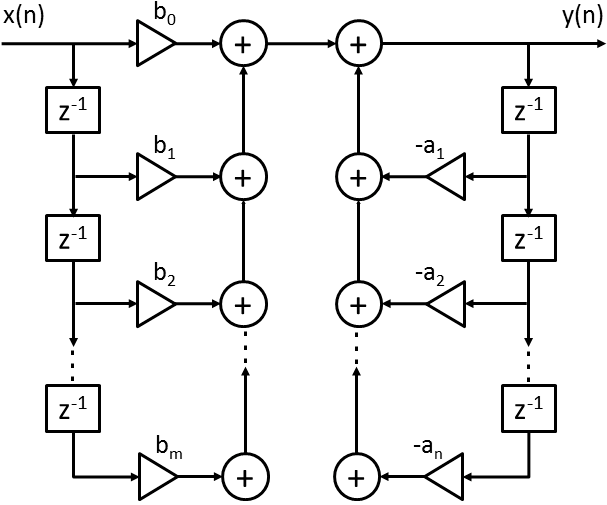
\includegraphics[width=0.85\linewidth]{images/direct_form_I.png}
\end{center}

Nachteil:
\begin{itemize}
\item Zwei getrennte Delay-Ketten
\item Höherer Speicherbedarf
\end{itemize}

%%%%%%%%%%%%%%%%%%%%%%%%%%%%%%%%%%%%%%%%%%%%%%%%%%%%%%%%%%%%
\subsection{Direct Form II (Canonical Form)}

Idee:  
Gemeinsame Nutzung der Delay-Elemente.

Zerlegung:

\[
H(z)=N(z)\cdot\frac{1}{D(z)}
\]

Zustandsgleichung:

\[
w(n)=x(n)-\sum_{k=1}^{M} a_k w(n-k)
\]

Ausgang:

\[
y(n)=\sum_{k=0}^{L} b_k w(n-k)
\]

Speicherbedarf:
\[
\max(L,M)
\]
\begin{center}
    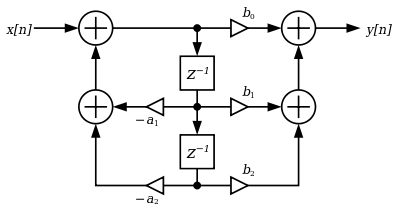
\includegraphics[width=0.85\linewidth]{images/direct_form_II.png}
\end{center}


Vorteil:
\begin{itemize}
\item Minimaler Speicher
\end{itemize}

Nachteil:
\begin{itemize}
\item Numerisch empfindlicher bei hoher Ordnung
\end{itemize}

%%%%%%%%%%%%%%%%%%%%%%%%%%%%%%%%%%%%%%%%%%%%%%%%%%%%%%%%%%%%
\subsection{Transposed Form}

Transformation eines Blockdiagramms:

\begin{itemize}
\item Addierer $\leftrightarrow$ Verzweigungen
\item Signalflussrichtung umkehren
\item Eingang und Ausgang vertauschen
\end{itemize}

\begin{center}
    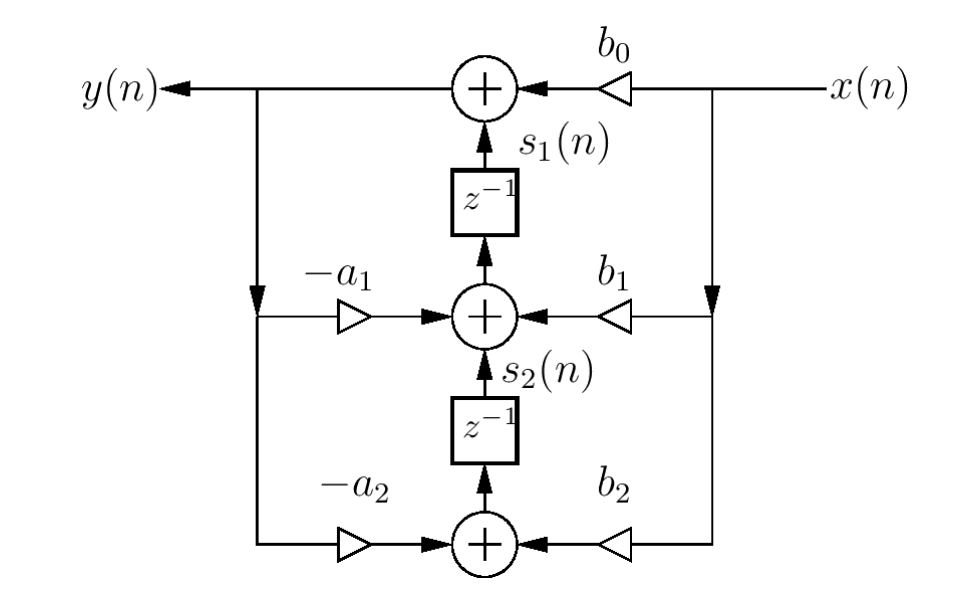
\includegraphics[width=0.85\linewidth]{images/transposed_form.png}
\end{center}



Eigenschaft:
\[
H(z) \text{ bleibt unverändert}
\]

Oft bessere numerische Eigenschaften bei Festkomma.

%%%%%%%%%%%%%%%%%%%%%%%%%%%%%%%%%%%%%%%%%%%%%%%%%%%%%%%%%%%%
\subsection{Parallel Form}

Mittels Partialbruchzerlegung:

\[
H(z)=\sum_i \frac{A_i}{1-p_i z^{-1}}
\]

Implementierung:

\begin{itemize}
\item Mehrere Teilsysteme
\item Ausgang = Summe der Teiloutputs
\end{itemize}

Vorteil:
\begin{itemize}
\item Gute Interpretierbarkeit einzelner Pole
\end{itemize}

%%%%%%%%%%%%%%%%%%%%%%%%%%%%%%%%%%%%%%%%%%%%%%%%%%%%%%%%%%%%
\subsection{Cascade Form (Second Order Sections)}

Faktorisierung:

\[
H(z)=\prod_{i=1}^{K}
\frac{b_{0i}+b_{1i}z^{-1}+b_{2i}z^{-2}}
{1+a_{1i}z^{-1}+a_{2i}z^{-2}}
\]

Vorgehen:

\begin{enumerate}
\item Nullstellen berechnen
\item Pole berechnen
\item Komplexe konjugierte Paare bilden
\item Reelle Wurzeln paarweise kombinieren
\item Jede Sektion in Canonical Form implementieren
\end{enumerate}

\begin{center}
    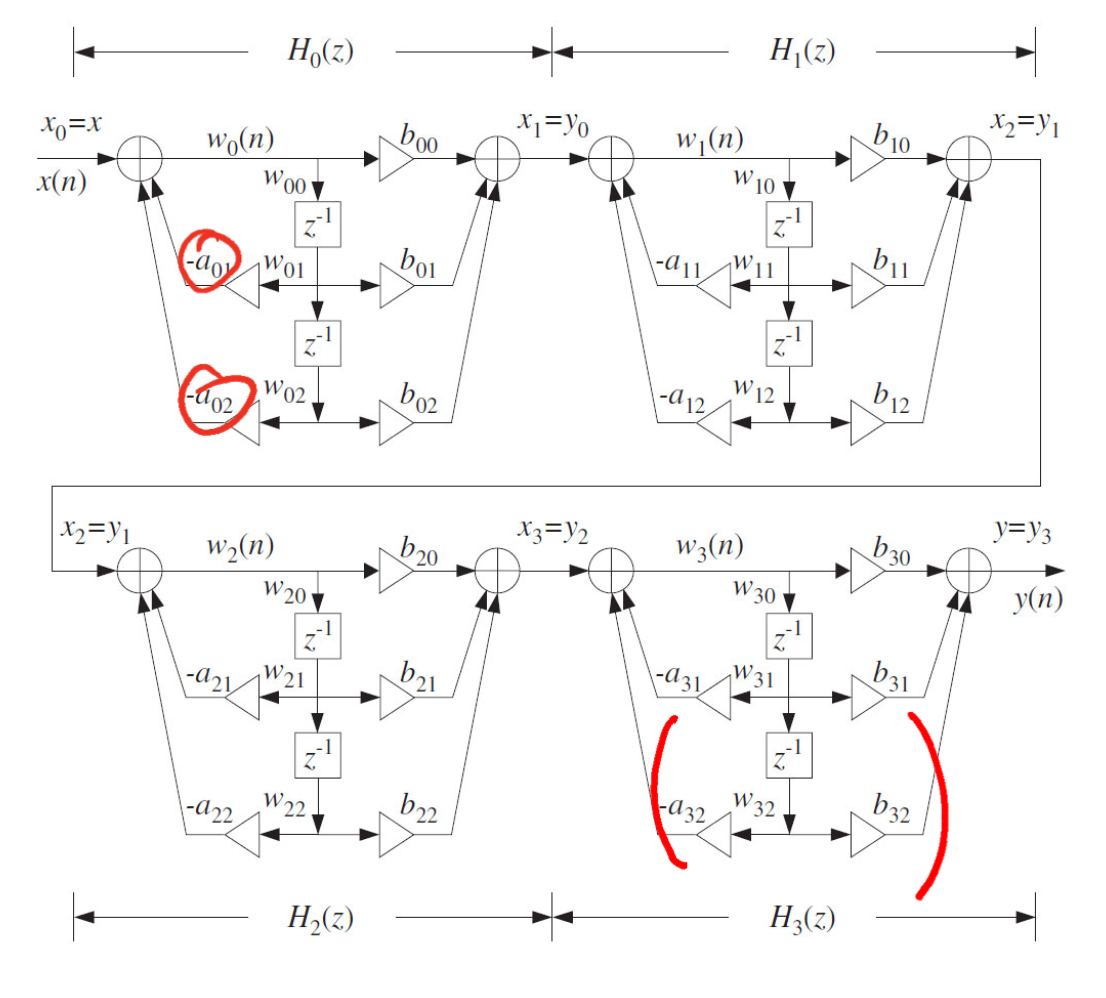
\includegraphics[width=0.85\linewidth]{images/cascade_form.png}
\end{center}

Vorteil:
\begin{itemize}
\item Deutlich bessere numerische Stabilität
\item Standard bei hoher Ordnung
\end{itemize}

%%%%%%%%%%%%%%%%%%%%%%%%%%%%%%%%%%%%%%%%%%%%%%%%%%%%%%%%%%%%
\subsection{DC-Gain}

\[
H(1)=\frac{\sum_{k=0}^{L} b_k}
{1+\sum_{k=1}^{M} a_k}
\]

%%%%%%%%%%%%%%%%%%%%%%%%%%%%%%%%%%%%%%%%%%%%%%%%%%%%%%%%%%%%
\subsection{Hardware Realization and Circular Buffers}

Digitale Implementierung:

\begin{itemize}
\item Multiply-Accumulate (MAC)
\item Koeffizienten in Speicher
\item Zustände in RAM
\end{itemize}

Circular Buffer Prinzip:

\begin{itemize}
\item Kein physisches Verschieben der Samples
\item Ringstruktur
\item Nur Index wird rotiert
\item Echtzeitfähig
\end{itemize}

%%%%%%%%%%%%%%%%%%%%%%%%%%%%%%%%%%%%%%%%%%%%%%%%%%%%%%%%%%%%
\subsection{Quantization Effects}

Endliche Wortlänge führt zu:

\begin{itemize}
\item Polverschiebung
\item Instabilität
\item Rundungsrauschen
\item Limit Cycles
\end{itemize}

Robusteste Struktur:
\[
\text{Second Order Sections}
\]

%%%%%%%%%%%%%%%%%%%%%%%%%%%%%%%%%%%%%%%%%%%%%%%%%%%%%%%%%%%%

